\documentclass[tikz]{standalone}
    \usepackage{tikz}
    \usetikzlibrary{positioning, graphs}
    \usetikzlibrary{graphs.standard}
    \begin{document}
    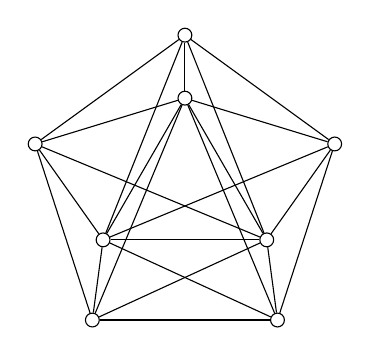
\begin{tikzpicture}
            [every node/.style={draw,circle,inner sep = 0mm, minimum size = 0.5em}]
            \graph[clockwise, phase = 90, empty nodes]{
                subgraph C_n[n = 5, name = A, radius = 2cm] --[complete bipartite]
                subgraph C_n[n = 3, name = B, radius = 0.2cm]
            };
    \end{tikzpicture}
    \end{document}